% !TEX root = ../main.tex
\chapter{Simulating Continuous and Discrete Dynamics}\label{ch:simulation}
\begin{paracol}{2}

\begin{sources}
\begin{tabularx}{\linewidth}{@{}V l L@{}}
\toprule
\textbf{Video} & \textbf{Length} & \textbf{Content}\\
\midrule
\seg{3}{1}{V3.1 Simulating the Lorenz System in Matlab} & 15:09 & The Lorenz equations; coding the right-hand side; \texttt{ode45} with tight tolerances; plotting the butterfly; a blob of initial conditions stretched and folded.\\
\seg{3}{2}{V3.2 Discrete-Time Dynamical Systems} & 9:46 & From $\dot{\vb x}=\vb f(\vb x)$ to $\vb x_{k+1}=\vb F(\vb x_k)$: sampling, the flow map; maps are more general; forward Euler as a crude flow map; preview of the logistic map.\\
\seg{3}{3}{V3.3 Simulating the Logistic Map in Matlab} & 16:29 & Iterating $x_{k+1}=\beta x_k(1-x_k)$ for $\beta\in[0,4]$; removing transients; the bifurcation diagram (``mathematical mountains''); the logistic model of a population.\\
\bottomrule
\end{tabularx}

\smallskip
\textbf{Transcripts} \file{materials/transcripts/C03-V0*.txt}.
\textbf{Book} Sec.~7.1 (Lorenz code, logistic map, Fig.~7.1--7.2).
\textbf{Code} \file{code/ch03_lorenz.py}, \file{ch03_euler.py}, \file{ch03_logistic.py} (the Matlab of
the videos rewritten in Python; run from the repository root, they regenerate the figures).
\end{sources}

\section*{Motivation}
Three practical videos. The point is not the code itself but what it will be used for: simulated
trajectories of systems like Lorenz are the \emph{data} on which every method of the course (DMD,
SINDy, Koopman, HAVOK) is tested \ts{3}{1}{14:36}. On the way, the second video makes precise the
relation between continuous and discrete time, which matters because data always come sampled.

% ------------------------------------------------------------------
\section{Simulating the Lorenz system}\label{sec:si-lorenz}

The Lorenz system (1963) is one of the earliest models of chaos: a three-dimensional caricature of
turbulent atmospheric convection \ts{3}{1}{0:43}:
\begin{equation}\label{eq:si-lorenz}
  \dot x=\sigma(y-x),\qquad \dot y=x(\rho-z)-y,\qquad \dot z=xy-\beta z ,
\end{equation}
with state $\vb x=(x,y,z)^{\mathsf T}$ and parameter vector $\boldsymbol\beta=(\sigma,\rho,\beta)^{\mathsf T}$
\ts{3}{1}{1:03}\ts{3}{1}{1:45}. The classic chaotic values used by Lorenz are $\sigma=10$, $\rho=28$,
$\beta=8/3$ \ts{3}{1}{6:58}. A trajectory oscillates around one lobe, jumps to the other, oscillates
there, and so on \ts{3}{1}{2:27}.

\begin{secondary}[What the Lorenz variables are]
Lorenz truncated the Boussinesq equations of a fluid layer heated from below (Rayleigh--B\'enard
convection, following B.~Saltzman 1962) to three Fourier modes: $x$ is the intensity of the convective
roll, $y$ the temperature difference between rising and falling fluid, $z$ the distortion of the
vertical temperature profile. $\sigma$ is the Prandtl number, $\rho$ the Rayleigh number divided by its
critical value, $\beta$ a geometric factor. Fixed points: the origin (conduction) and, for $\rho>1$, the
two rolls $C_\pm=\big(\pm\sqrt{\beta(\rho-1)},\pm\sqrt{\beta(\rho-1)},\rho-1\big)$, the centres of the two
lobes; for $\sigma=10$, $\beta=8/3$ they lose stability in a subcritical Hopf bifurcation at
$\rho\approx24.74$, so at $\rho=28$ all three fixed points are unstable.
\end{secondary}

\paragraph{The recipe.} Everything is in three steps \ts{3}{1}{13:34}:
\begin{enumerate}
  \item code the right-hand side $\vb f(t,\vb x;\boldsymbol\beta)$ as a function. The integrator wants a
        function of $(t,\vb x)$ even when $\vb f$ does not depend on $t$; the parameters are ``locked in''
        by wrapping it (in Matlab \texttt{@(t,x) lorenz(t,x,Beta)}, in Python \texttt{args=(beta,)})
        \ts{3}{1}{3:08}\ts{3}{1}{8:42}\ts{3}{1}{9:23};
  \item choose parameters, initial condition $\vb x_0=(0,1,20)$, time step $\Delta t=0.001$ and span up to
        $t=50$, i.e.\ $50\,000$ samples \ts{3}{1}{7:20}\ts{3}{1}{7:40};
  \item call an adaptive Runge--Kutta integrator (Matlab \texttt{ode45}) with tight relative and absolute
        tolerances, $10^{-12}$: the integrator shrinks its internal step until the error estimate meets
        them \ts{3}{1}{10:05}\ts{3}{1}{10:49}. The output is a $50\,000\times3$ array: one column per
        variable, one row per time \ts{3}{1}{11:50}.
\end{enumerate}

\codefile{Lorenz attractor and a blob of initial conditions}{../code/ch03_lorenz.py}

\begin{coursenote}[Matlab and Python]
Matlab's \texttt{ode45} is the Dormand--Prince 5(4) pair; \texttt{scipy}'s equivalent is
\texttt{method='RK45'}. Here \texttt{DOP853} (order 8) is used because at tolerance $10^{-12}$ it is
much faster. \texttt{t\_eval} plays the role of \texttt{tspan}: the integrator chooses its own steps and
interpolates at the requested times.
\end{coursenote}

\begin{nfigure}
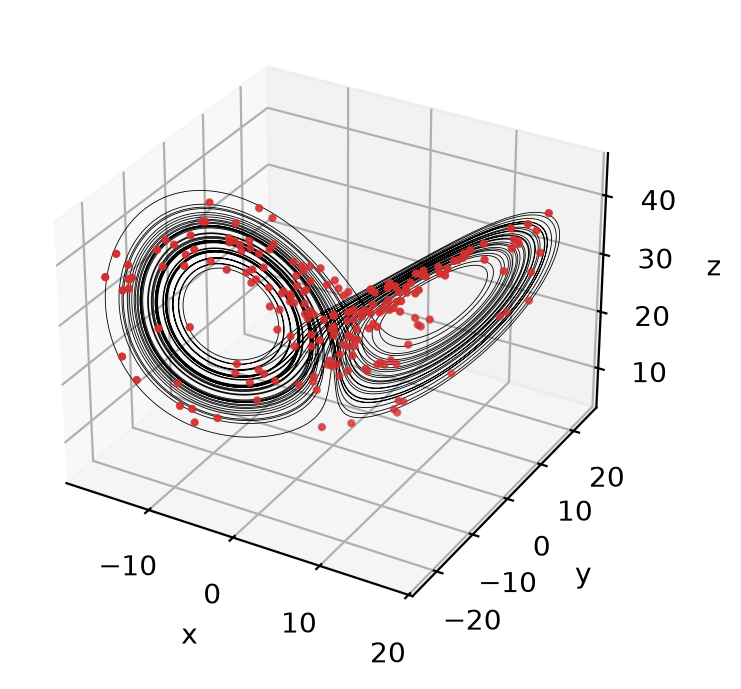
\includegraphics[width=0.55\linewidth]{figures/ch03-lorenz.png}
\caption{Output of \file{ch03_lorenz.py}: the Lorenz butterfly (black), and in red where 200 initial
conditions, all within $\sim10^{-3}$ of $\vb x_0$, are at $t=15$. They have spread over the whole
attractor (their range is $\sim35$--$45$ in each coordinate).}\label{fig:si-lorenz}
\end{nfigure}

\paragraph{Sensitive dependence.} Brunton closes with a movie of a small red blob of initial
conditions integrated through the system: it stretches, folds and mixes over the butterfly wings
\ts{3}{1}{13:55}\ts{3}{1}{14:15}. Any uncertainty in the initial condition grows exponentially; two points
starting very close end up far apart, and after long enough only a statistical description of where the
points are is possible \ts{3}{1}{14:36}. The red points of \cref{fig:si-lorenz} reproduce this.

% ------------------------------------------------------------------
\section{From continuous to discrete time}\label{sec:si-discrete}

A continuous-time system $\dot{\vb x}(t)=\vb f(\vb x(t))$ (the populations of a predator and a prey, or
anything else) \ts{3}{2}{0:01}\ts{3}{2}{0:22} induces a discrete-time system
$\vb x_{k+1}=\vb F(\vb x_k)$ \ts{3}{2}{1:03}. Usually $k$ is the step of an integrator, but it need not
be time at all \ts{3}{2}{1:23}. Sampling every $\Delta t$ (say, counting a population once a day),
$\vb x_k=\vb x(k\Delta t)$, and $\vb F$ is the flow map of \cref{def:fu-flowmap}
\ts{3}{2}{1:43}\ts{3}{2}{2:04}:
\begin{equation}\label{eq:si-flowmap}
  \vb x_{k+1}=\vb F_{\Delta t}(\vb x_k)=\vb x_k+\int_{k\Delta t}^{(k+1)\Delta t}\vb f(\vb x(\tau))\,\mathrm d\tau ,
\end{equation}
where the state inside the integral moves along the trajectory \ts{3}{2}{2:25}\ts{3}{2}{3:08}\ts{3}{2}{3:50}.

\begin{proposition}[Maps are more general than flows]
Every continuous-time system defines a discrete-time one through \eqref{eq:si-flowmap}, but not every
map is the flow map of some ODE \ts{3}{2}{4:10}\ts{3}{2}{4:32}.
\end{proposition}
Real populations, with seasons and other discrete events, are naturally maps \ts{3}{2}{4:52}. A
mathematical obstruction: a flow map $\vb F_{\Delta t}=\vb F_{\Delta t/2}\circ\vb F_{\Delta t/2}$ is a
diffeomorphism isotopic to the identity, so in one dimension it is increasing; the logistic map, which
is not invertible, cannot be the flow map of any one-dimensional ODE (a one-dimensional ODE cannot even
oscillate, let alone be chaotic).

\paragraph{Forward Euler as a crude flow map.} Replace the derivative by a finite difference
\ts{3}{2}{5:13}\ts{3}{2}{5:34}:
\[
  \frac{\vb x_{k+1}-\vb x_k}{\Delta t}\approx\vb f(\vb x_k)
  \quad\Longrightarrow\quad
  \vb x_{k+1}=\vb x_k+\Delta t\,\vb f(\vb x_k) .
\]
This is \eqref{eq:si-flowmap} with the integral approximated by a left rectangle: $\vb f$ held constant
over the step \ts{3}{2}{6:16}\ts{3}{2}{6:57}. Runge--Kutta schemes are better approximations of the same
true flow map \ts{3}{2}{7:38}. Only a handful of systems have a closed-form flow map, notably the linear
ones, $\vb F_t=e^{At}$; in general it must be approximated numerically \ts{3}{2}{7:59}.

\begin{proposition}[Order of Euler and RK4]\label{prop:si-order}
For smooth $\vb f$ the local error of one Euler step is $O(\Delta t^2)$ and the global error at a fixed
final time is $O(\Delta t)$; for the classical fourth-order Runge--Kutta scheme they are $O(\Delta t^5)$
and $O(\Delta t^4)$.
\end{proposition}
\begin{proof}
Taylor: $\vb x(t+\Delta t)=\vb x+\Delta t\,\vb f+\tfrac12\Delta t^2\,D\vb f\,\vb f+O(\Delta t^3)$; Euler
keeps the first two terms, so its local error is $\tfrac12\Delta t^2 D\vb f\,\vb f$. Over $N=T/\Delta t$
steps the local errors add up (each amplified at most by $e^{LT}$, $L$ the Lipschitz constant), giving
$N\cdot O(\Delta t^2)=O(\Delta t)$. RK4 matches the Taylor series up to $\Delta t^4$ (one checks it
term by term), hence local $O(\Delta t^5)$, global $O(\Delta t^4)$.
\end{proof}

\codefile{Euler and RK4 against the exact flow map}{../code/ch03_euler.py}

For the harmonic oscillator over one period the script prints, for $\Delta t\approx0.1,0.01,0.001$:
Euler errors $3.7\times10^{-1}$, $3.2\times10^{-2}$, $3.1\times10^{-3}$ (a factor 10 per factor 10 in
$\Delta t$: first order); RK4 errors $5.2\times10^{-6}$, $5.2\times10^{-10}$, $5.3\times10^{-14}$ (a
factor $10^4$: fourth order).

\begin{example}[Euler spirals outward]
For $\dot{\vb x}=A\vb x$ with $A=\begin{psmallmatrix}0&1\\-1&0\end{psmallmatrix}$ Euler gives
$\vb x_{k+1}=(I+\Delta tA)\vb x_k$, whose eigenvalues $1\pm i\Delta t$ have modulus
$\sqrt{1+\Delta t^2}>1$: the discrete orbit spirals out, energy grows by a factor
$(1+\Delta t^2)$ per step, while the true eigenvalues $e^{\pm i\Delta t}$ lie on the unit circle.
\end{example}

% ------------------------------------------------------------------
\section{The logistic map}\label{sec:si-logistic}

\paragraph{The model.} The logistic map
\begin{equation}\label{eq:si-logistic}
  x_{k+1}=\beta x_k(1-x_k)
\end{equation}
is a crude model of a population \ts{3}{2}{8:40}\ts{3}{3}{14:39}. Start from exponential growth,
$x_{k+1}=\beta x_k$; resources are finite, so with a carrying capacity normalized to 1 the growth factor
must go to zero as $x\to1$; multiplying by $(1-x_k)$ does that \ts{3}{3}{14:59}\ts{3}{3}{15:20}. It has
fixed points for zero and for ``full'' population, and as $\beta$ is turned up it becomes chaotic
\ts{3}{2}{9:01}\ts{3}{2}{9:22}.

\paragraph{The algorithm} \ts{3}{3}{1:03}\ts{3}{3}{1:45}:
\begin{enumerate}
  \item for each $\beta$ on a grid from $0$ to $4$, start from $x_0=0.5$;
  \item iterate a few thousand times without saving, to remove the transient and land on the attractor
        \ts{3}{3}{2:26}\ts{3}{3}{3:28};
  \item iterate up to a thousand more times, saving the pairs $(\beta,x_k)$; stop early if $x_k$ returns
        within $10^{-3}$ of the first saved value (a fixed point or a short periodic orbit needs no more
        points) \ts{3}{3}{3:49}\ts{3}{3}{4:52}\ts{3}{3}{5:12};
  \item scatter-plot all the pairs: the \emph{bifurcation diagram} \ts{3}{3}{5:54}.
\end{enumerate}

\codefile{bifurcation diagram of the logistic map}{../code/ch03_logistic.py}

\begin{coursenote}[Operator precedence]
In the video the update is written as ``\texttt{xold - xold\^{}2} times beta'', i.e.\
$(x-x^2)\beta=\beta x(1-x)$. Typed literally as \texttt{x - x**2*beta} it would be the map
$x-\beta x^2$, which is conjugate to the logistic map at fixed parameter 1 and never becomes chaotic
(and for $\beta>2$ leaves $[0,1]$ and diverges): a bug made, and caught, while writing these notes.
\end{coursenote}

\begin{nfigure}
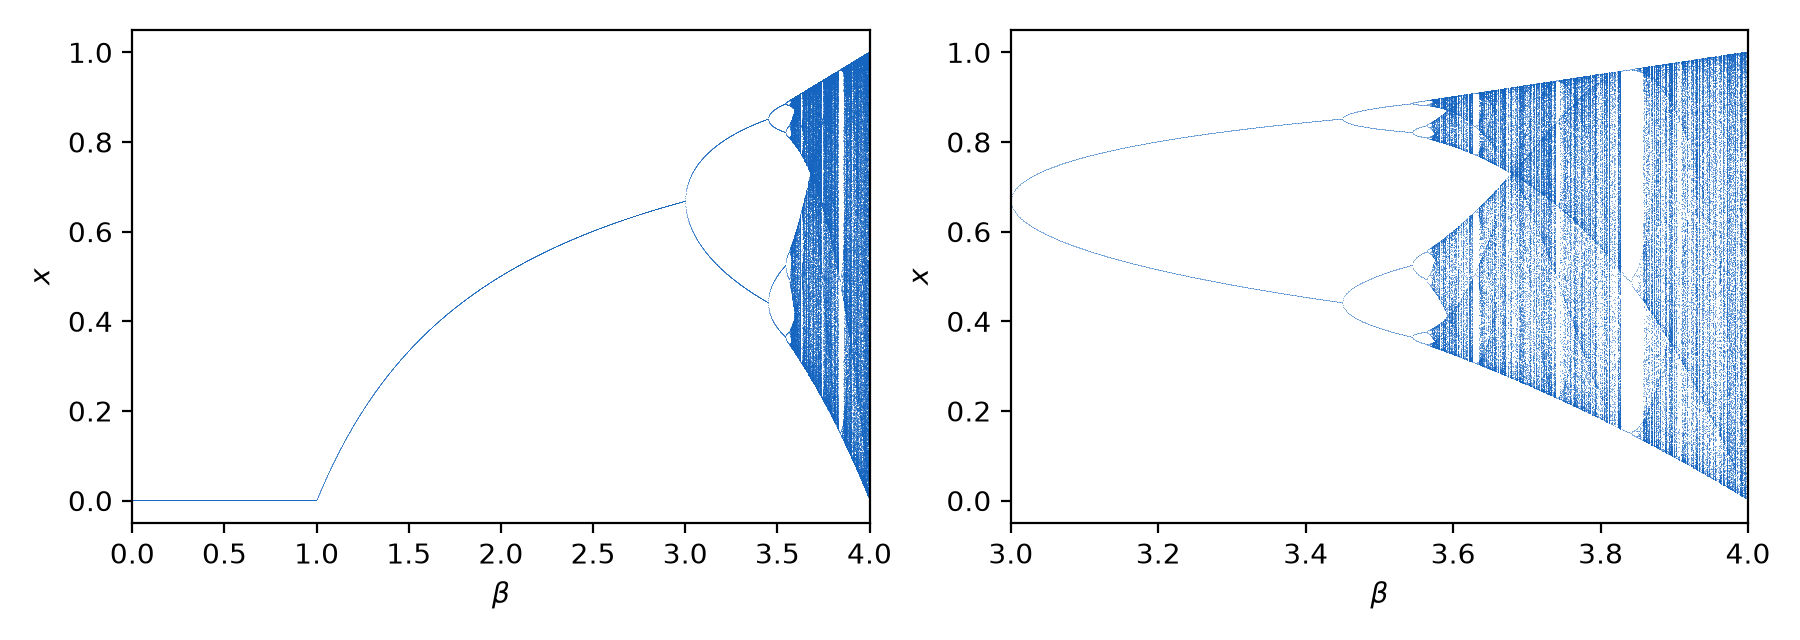
\includegraphics[width=\linewidth]{figures/ch03-logistic.png}
\caption{Output of \file{ch03_logistic.py}: bifurcation diagram of the logistic map (left, $\beta\in[0,4)$)
and zoom on $\beta\in[3,4]$ (right). In the video the axes are flipped so that the picture looks like
mountains, ``mathematical mountains'' \ts{3}{3}{8:43}\ts{3}{3}{13:57}.}\label{fig:si-logistic}
\end{nfigure}

\paragraph{Reading the diagram} \ts{3}{3}{7:20}:
\begin{itemize}
  \item $0\le\beta<1$: every orbit goes to $x=0$, the population dies out;
  \item $1<\beta<3$: a single nonzero fixed point, reached after a transient and kept forever
        \ts{3}{3}{7:40};
  \item at $\beta=3$ the fixed point splits into two values visited alternately, a period-2 orbit:
        the population is bigger, smaller, bigger, smaller from one generation to the next
        \ts{3}{3}{8:02};
  \item increasing $\beta$ the period doubles again, to 4 (Brunton calls it ``quasi periodic'', but it
        is a period-4 orbit), then 8, 16, \dots\ \ts{3}{3}{8:22};
  \item between about $3.57$ and $4$ the system is chaotic, with windows of periodic behaviour (the
        clear window near $\beta\approx3.83$ is a period-3 orbit) \ts{3}{3}{8:22}\ts{3}{3}{13:16}.
\end{itemize}
Keeping the transients in the plot shows the lines along which $x$ jumps from $0.5$ to the attractor
\ts{3}{3}{11:08}\ts{3}{3}{11:52}; that is why they are usually removed \ts{3}{3}{12:14}.

\begin{proposition}[First two bifurcations]\label{prop:si-logistic}
For \eqref{eq:si-logistic}, $F(x)=\beta x(1-x)$:
\begin{enumerate}[(i)]
  \item the fixed points are $x=0$ and $x^*=1-1/\beta$; $x=0$ is stable for $\beta<1$, and $x^*$ is
        stable for $1<\beta<3$;
  \item at $\beta=3$, $F'(x^*)=-1$ and a stable period-2 orbit is born (period-doubling, or
        \emph{flip}, bifurcation); it is stable for $3<\beta<1+\sqrt6\approx3.449$.
\end{enumerate}
\end{proposition}
\begin{proof}
A fixed point of a map is stable if $|F'(x^*)|<1$ (the linearization of $x_{k+1}=F(x_k)$ is
$\Delta x_{k+1}=F'(x^*)\Delta x_k$). $F'(x)=\beta(1-2x)$, so $F'(0)=\beta$ and
$F'(x^*)=\beta(1-2+2/\beta)=2-\beta$, with $|2-\beta|<1\iff1<\beta<3$. At $\beta=3$ the multiplier
crosses $-1$: deviations alternate in sign without decaying. The period-2 points solve $F(F(x))=x$; dividing
out the fixed points leaves $\beta^2x^2-\beta(\beta+1)x+(\beta+1)=0$, real for $\beta>3$; the multiplier of
the orbit is $F'(x_1)F'(x_2)=-\beta^2+2\beta+4$, which equals $-1$ at $\beta=1+\sqrt6$.
\end{proof}

\begin{intuition}[Faster growth, more chaos]
The moral Brunton draws from this crude model: the faster the growth rate, the more erratic the
population; ``breakneck population growth'' is a bad idea \ts{3}{3}{15:41}\ts{3}{3}{16:02}. The physical
reason is overshoot: with a large $\beta$ a big population produces a crash the next year, and the
discrete delay (one generation) turns a smooth relaxation into oscillations.
\end{intuition}

\begin{history}[May, Feigenbaum and universality]
The ecologist Robert May made the logistic map famous with \emph{Simple mathematical models with very
complicated dynamics}, Nature 261 (1976) 459--467, a plea to teach students that simple nonlinear maps
can be chaotic. Mitchell Feigenbaum (Los Alamos, 1975--78) found, at first with an HP-65 pocket
calculator, that the parameter values of successive period doublings converge geometrically with ratio
$\delta=4.6692\ldots$, the \emph{same} for every map with a quadratic maximum: a universal constant,
later explained by renormalization. Libchaber and Maurer saw the cascade in convecting liquid helium in
1980.\par
\textit{References:} R.~M.~May, Nature 261 (1976); M.~J.~Feigenbaum, J.\ Stat.\ Phys.\ 19 (1978) 25--52;
S.~Strogatz, \emph{Nonlinear Dynamics and Chaos}, ch.~10.
\end{history}

\begin{keyformulas}
\begin{itemize}
  \item Lorenz: $\dot x=\sigma(y-x)$, $\dot y=x(\rho-z)-y$, $\dot z=xy-\beta z$; $(10,28,8/3)$; $\vb x_0=(0,1,20)$.
  \item Flow map $\vb x_{k+1}=\vb x_k+\int_{k\Delta t}^{(k+1)\Delta t}\vb f(\vb x(\tau))\dd\tau$; Euler
        $\vb x_{k+1}=\vb x_k+\Delta t\vb f(\vb x_k)$, global error $O(\Delta t)$; RK4 $O(\Delta t^4)$.
  \item Logistic $x_{k+1}=\beta x_k(1-x_k)$: $x^*=1-1/\beta$ stable for $1<\beta<3$; period doubling at
        $3$, $1+\sqrt6$, \dots; chaos beyond $\approx3.57$.
\end{itemize}
\end{keyformulas}

\section*{Exercises}

\begin{exercise}[Lorenz fixed points]
Find the fixed points of \eqref{eq:si-lorenz} for $\rho>1$ and compute the Jacobian at the origin.
Show that the origin is stable for $\rho<1$ and a saddle with a one-dimensional unstable manifold for
$\rho>1$. Show that the volume of phase space contracts at the constant rate
$\nabla\cdot\vb f=-(\sigma+1+\beta)$, and conclude that the attractor has zero volume.
\end{exercise}

\begin{exercise}[Two nearby trajectories]
Modify \file{ch03_lorenz.py} to integrate $\vb x_0$ and $\vb x_0+10^{-8}(1,0,0)$, and plot
$\log\lVert\delta\vb x(t)\rVert$. Fit the slope of the linear part: compare with the largest Lyapunov
exponent $\lambda_1\approx0.906$. Why does the curve saturate?
\end{exercise}

\begin{exercise}[Tolerance matters]
Integrate Lorenz to $t=50$ with \texttt{rtol} $=10^{-3},10^{-6},10^{-9},10^{-12}$ and compare the final
states. Up to which time do the trajectories agree? Relate this to the prediction horizon of
Chapter~2.
\end{exercise}

\begin{exercise}[Backward Euler]
For $\dot{\vb x}=A\vb x$, backward Euler is $\vb x_{k+1}=(I-\Delta tA)^{-1}\vb x_k$. Compute its eigenvalues
for the harmonic oscillator and show that it spirals \emph{inward}. Which combination of forward and
backward Euler (the trapezoidal rule) preserves $|\mu|=1$ exactly?
\end{exercise}

\begin{exercise}[Period three]
Plot $F^3(x)-x$ for the logistic map near $\beta=1+\sqrt8\approx3.828$ and show that a pair of period-3
orbits is born there in a saddle-node (tangent) bifurcation. Run \file{ch03_logistic.py} zoomed on
$[3.82,3.86]$ and describe what happens at the edges of the window. (Li and Yorke, 1975: ``period
three implies chaos''.)
\end{exercise}

\begin{exercise}[Feigenbaum's constant]
Using bisection on the multiplier of the period-$2^n$ orbit, or by reading the zoomed bifurcation
diagram, estimate the first four period-doubling values $\beta_1=3$, $\beta_2\approx3.449$, $\beta_3$,
$\beta_4$, and the ratios $(\beta_n-\beta_{n-1})/(\beta_{n+1}-\beta_n)$.
\end{exercise}

\end{paracol}
